\subsection{Übung}

\subsubsection*{Aufgabe (Immatrikulationsprozess)}
    \paragraph*{Aufgabe}
        Modellieren Sie den im Folgenden beschriebenen Immatrikulationsprozess.
        Der Immatrikulationsprozess beginnt, nachdem der Immatrikulationsantrag eingegangen ist. Anschließend werden gleichzeitig die eingereichten Zeugnisse und die allgemeinen Angaben des Studenten geprüft. Erst nachdem beide Prüfungen abgeschlossen sind, wird über den Immatrikulationsantrag entschieden. Wenn die Immatrikulation abgelehnt wird, wird der Student über die Ablehnung informiert und der Prozess endet. Wenn dem Antrag stattgegeben wird, wird der Student im Prüfungssystem angelegt und der Student anschließend über den angenommenen Antrag informiert.
        \begin{figure}[h]
            \centering
            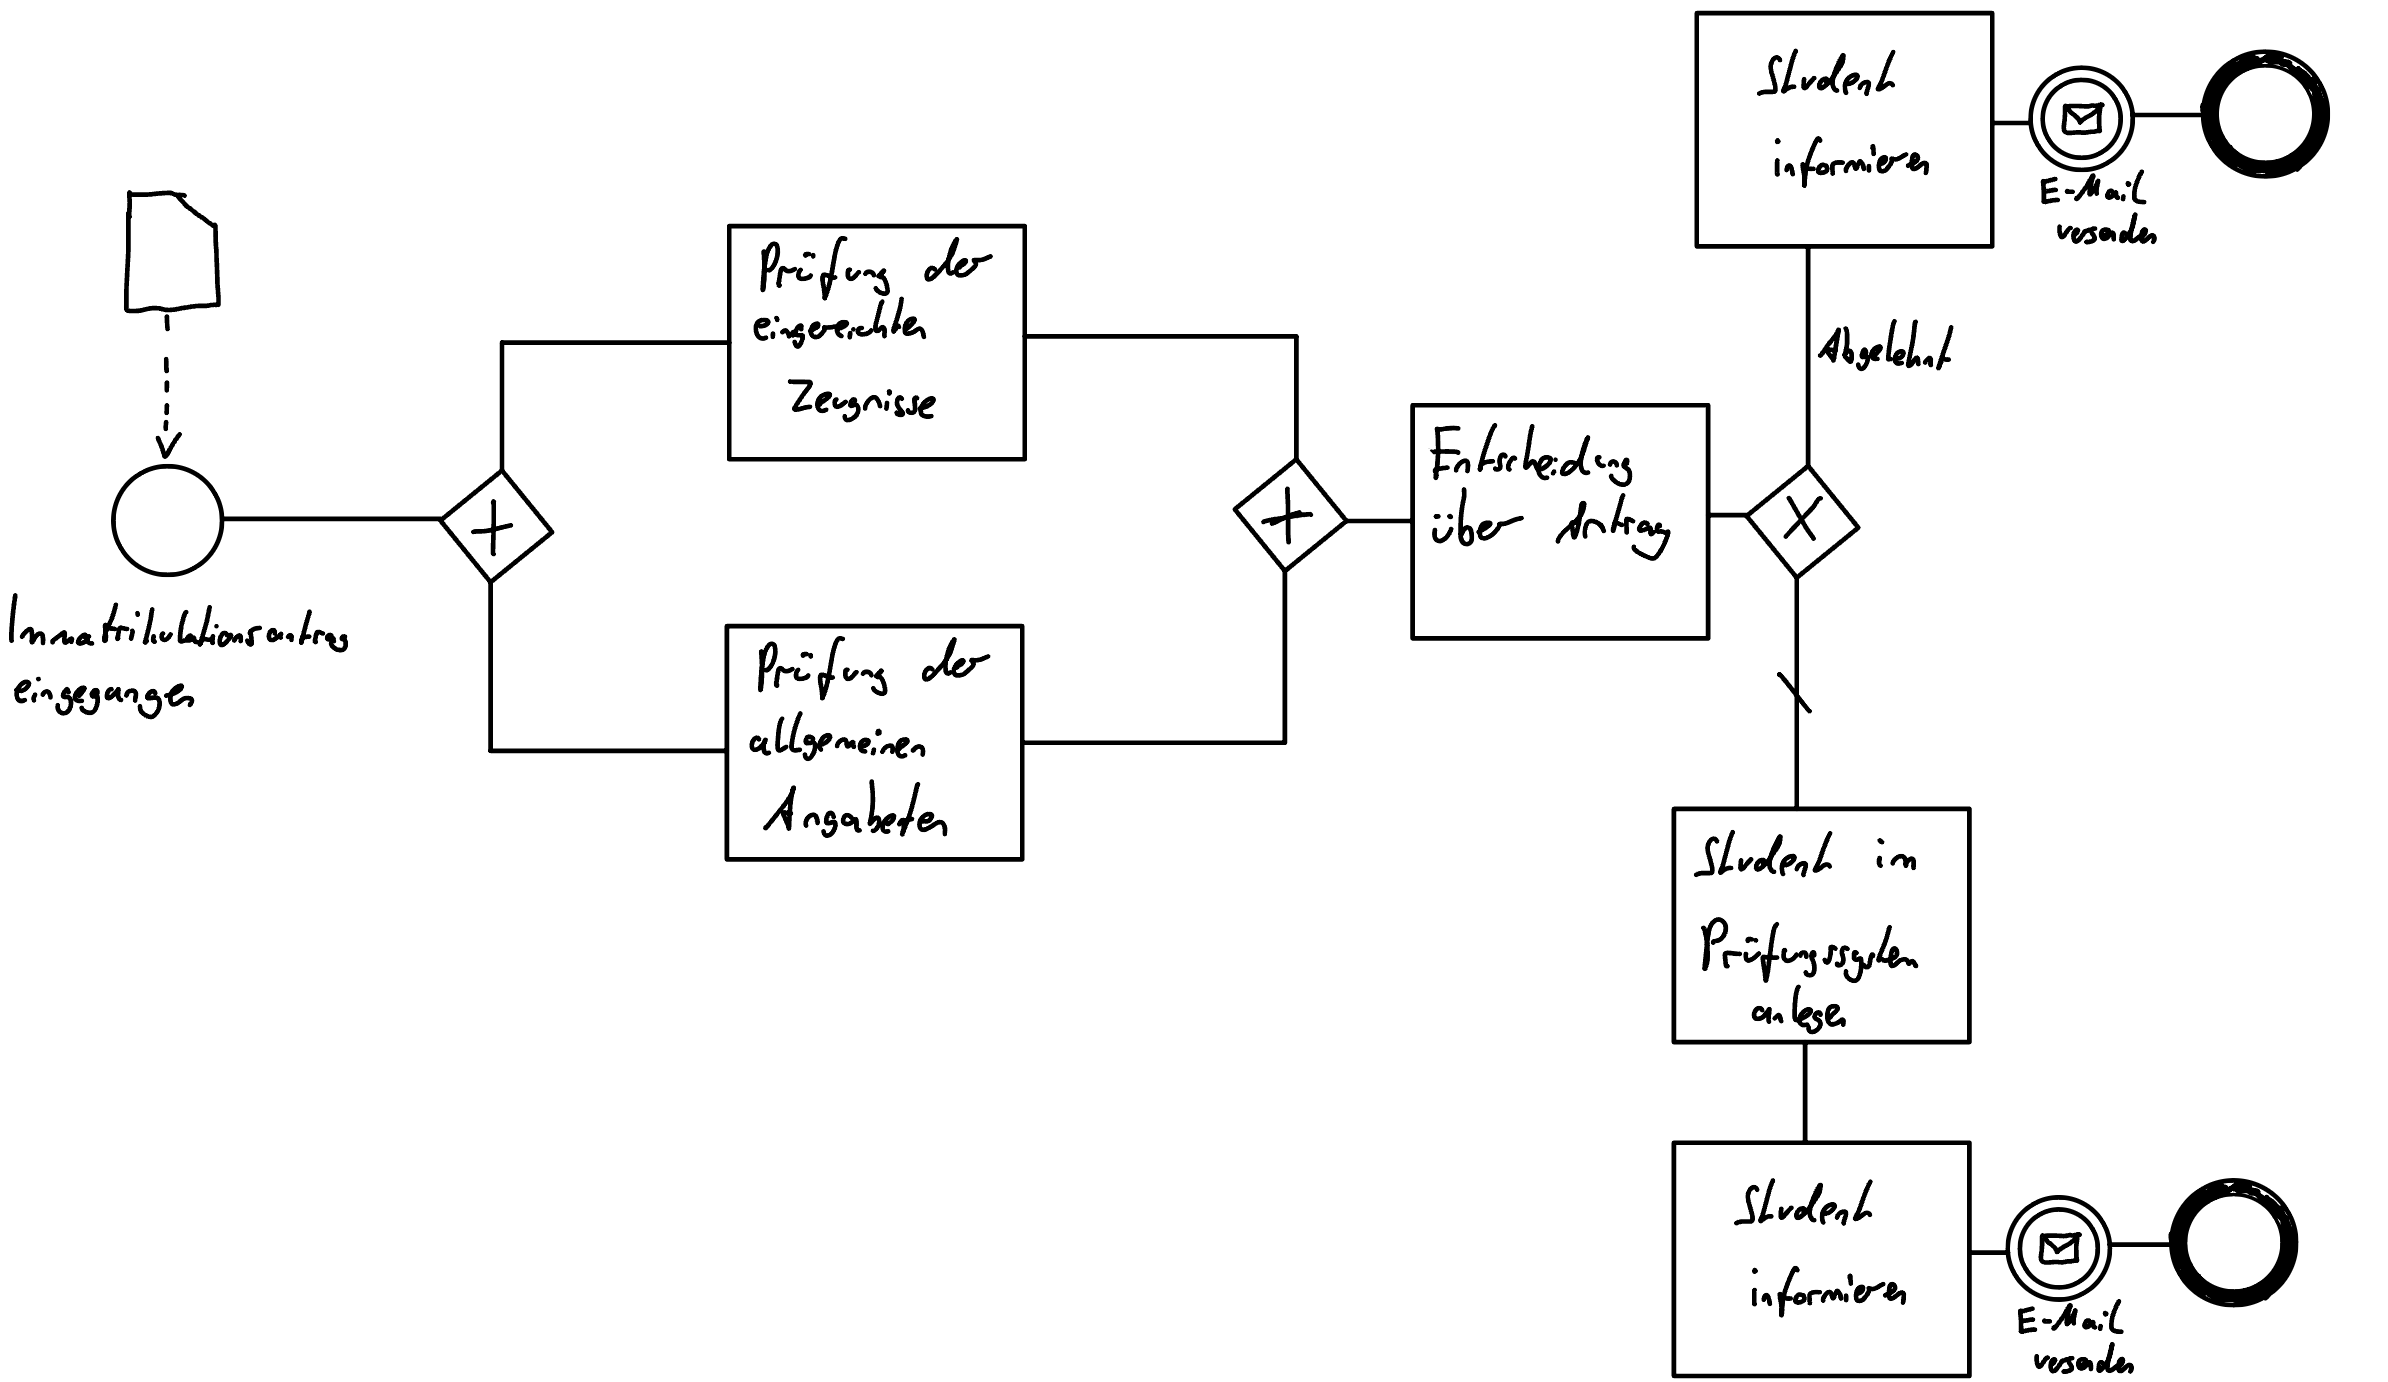
\includegraphics[width=\textwidth]{image/Loesung_Aufgabe_Immatrikulationsprozess.png}
            \caption{Lösung Aufgabe Immatrikulationsprozess}
            \label{fig:Loesung_Aufgabe_Immatrikulationsprozess}
        \end{figure}

\subsubsection*{Aufgabe (Prozess zur Zeugnisausstellung)}
    \paragraph*{Aufgabe}
        Modellieren Sie den im Folgenden beschriebenen Prozess zur Beantragung eines Zeugnisses. Der Prozess beginnt, nachdem der Antrag auf Zeugnisausstellung eingegangen ist. Im ersten Schritt werden die Prüfungsleistungen des Studierenden auf Vollständigkeit geprüft. Wenn
        die Prüfungsleistungen nicht vollständig sind, wird ein Bericht über die fehlenden Prüfungsleistungen erstellt und der Antrag anschließend abgelehnt. Wenn die Prüfungsleistungen vollständig sind, wird der Umfang der auszustellenden Unterlagen überprüft. Wenn der Student eine Leistungsübersicht wünscht, ist die Leistungsübersicht zu drucken. Wenn der Student die Bescheinigung eines Schwerpunkts wünscht, ist die Bescheinigung über den Schwerpunkt auszustellen. Parallel zur Erstellung
        der Leistungsübersicht und zur Erstellung der Schwerpunktbescheinigung wird das Zeugnis gedruckt und das Zeugnis dem Dekan zur Unterschrift vorgelegt. Nachdem alle erforderlichen Unterlagen erstellt wurden, werden diese an den Studierenden versendet.
        \begin{figure}[h]
            \centering
            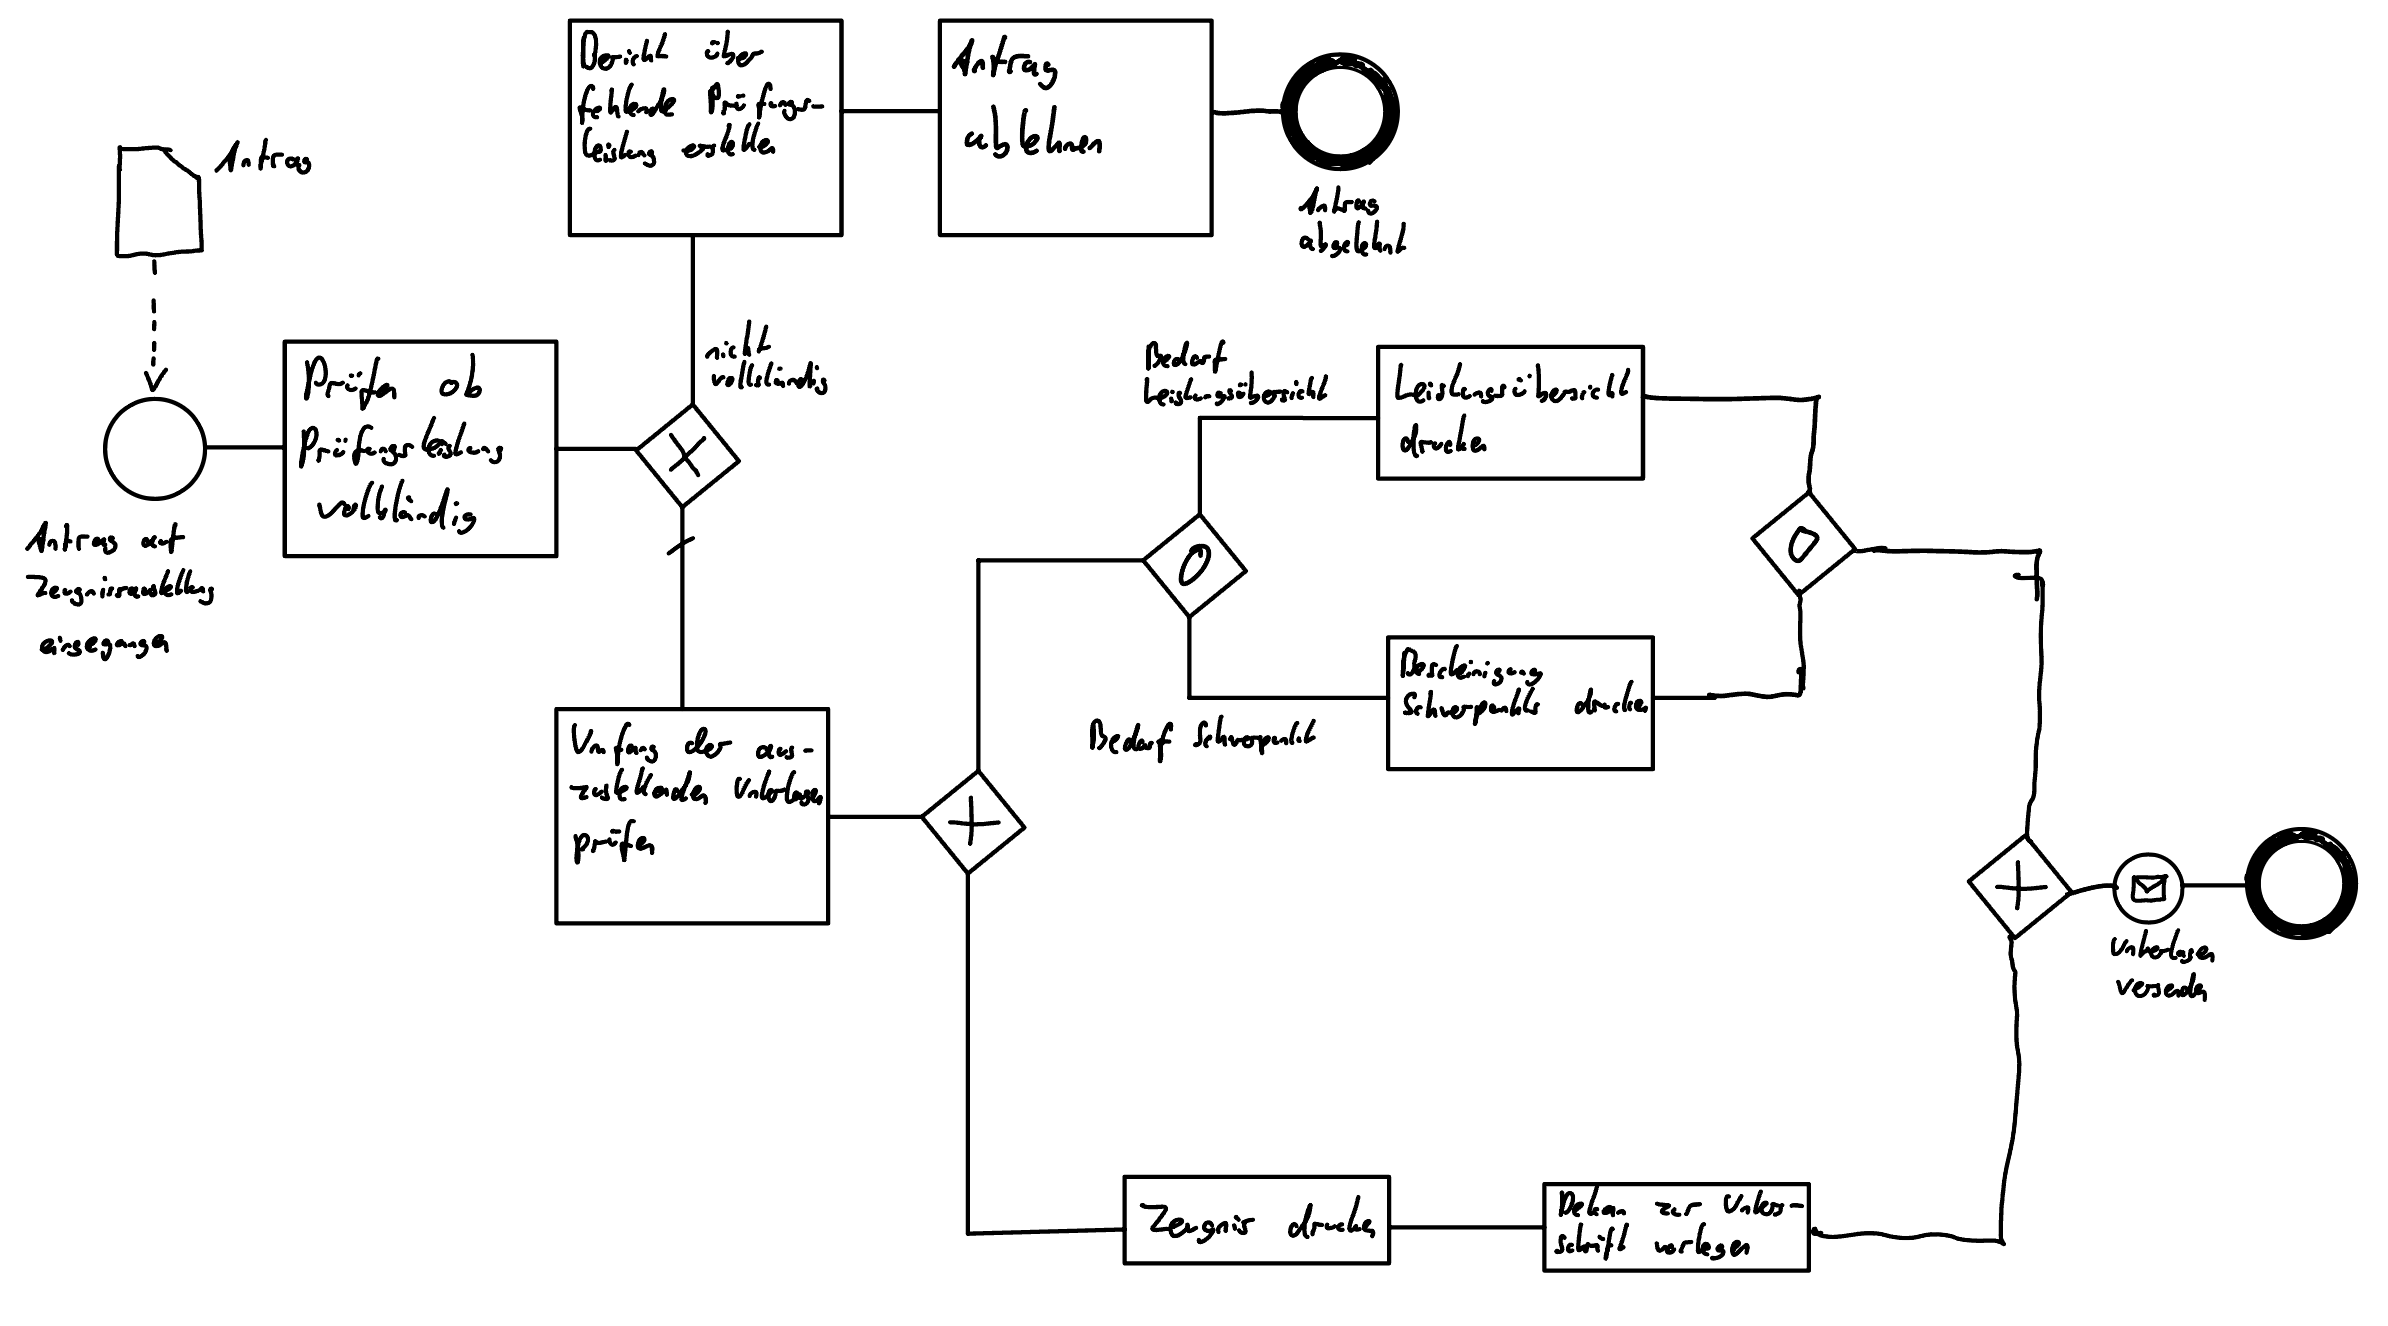
\includegraphics[width=\textwidth]{image/Loesung_Aufgabe_Prozess_zur_Zeugnissaustellung.png}
            \caption{Lösung Aufgabe Prozess zur Zeugnisausstellung}
            \label{fig:Loesung_Aufgabe_Prozess_zur_Zeugnissaustellung}
        \end{figure}

\subsubsection*{Aufgabe (Immatrikulationsprozess)}
    \paragraph*{Aufgabe}
        In der folgenden Abbildung ist eine im Vergleich zur Übungsaufgabe 5.1 weiter ausgearbeitete Version des Immatrikulationsprozesses dargestellt. Beachten Sie, dass im Schritt „Anlage des Studierenden im SVS“ der Antragsteller durch eine(n) Sachbearbeiter*in im „Studierendenverwaltungssystem“ (= SVS) angelegt wird.

        \begin{figure}[h]
            \centering
            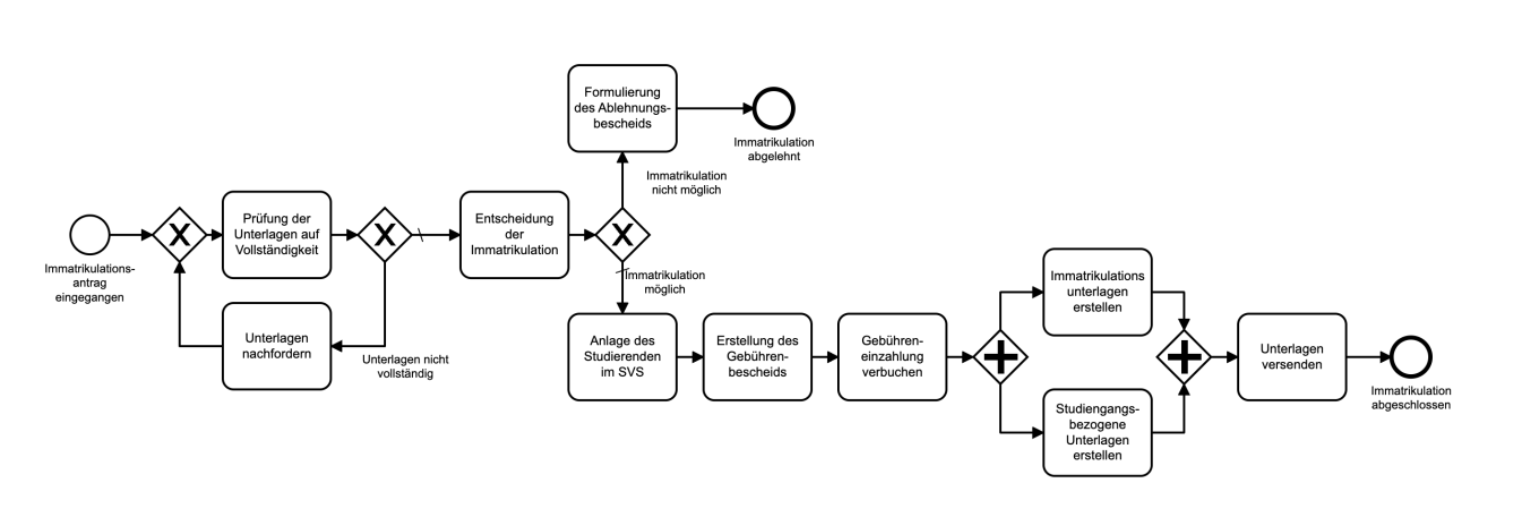
\includegraphics[width=\textwidth]{image/Aufgabe_6_1.png}
            \caption{Aufgabe Immatrikulationsprozess}
            \label{fig:Aufgabe_6_1}
        \end{figure}

        Machen Sie sich mit dem Prozess vertraut und beantworten Sie die folgenden Fragen:

        \begin{enumerate}[label=\alph*)]
            \item Warum darf das erste Gatter (XOR-Zusammenführung) nicht durch ein UND-Gatter ersetzt werden? Argumentieren Sie auf Basis der Schaltsemantik des UND-Gatters bei der Weiterschaltung von Marken.
            \item Hätte auf die Kantenbeschriftung „Immatrikulation möglich“ im Modell verzichtet werden können? Begründen Sie Ihre Aussage.
            \item Wo befinden sich die Marken zur Darstellung des Fortschritts einer Prozessinstanz, wenn die Immatrikulationsunterlagen bereits erstellt wurden und die Erstellung der studiengangsbezogenen Unterlagen zwar schon begonnen wurde aber noch nicht abgeschlossen ist?
        \end{enumerate}

    \paragraph*{Lösung}
        \begin{enumerate}[label=\alph*)]
            \item Wenn dort ein UND-Gatter wäre, dann wurde sich der Prozess teilen und eine Marke würde zu „Unterlagen anfordern“ gehen und eine zu „Entscheidung der Immatrikulation“. Außerdem würde es eine „loop“ geben.
            \item Ja, da der kleine Strich den Standartfluss kennzeichnet.
            \item Eine Marke an dem UND-Gatter, die andere am Beginn der Aktivität „Studienbezogene Unterlagen erstellen“.
        \end{enumerate}

\subsubsection*{Aufgabe (Fortgeschrittene Modellierung)}
    \paragraph*{Aufgabe}
        Gehen Sie von dem in Aufgabe 6.1 dargestellten Prozessmodell aus und erstellen Sie ein neues Modell, in dem Sie die folgenden Aspekte ergänzen bzw. ändern:

        \begin{itemize}
            \item Ergänzen Sie sinnvoll Datenobjekte und Datenspeicher, die bei der Ausführung des
            Prozesses benötigt werden.
            \item Ordnen Sie die Aktivitäten sinnvoll mindestens den beiden Ressourcenklassen
            „Sachbearbeiter*in“ und „Buchhaltung“ zu
            \item Identifizieren Sie einen Teilprozess „Unterlagen erstellen“ und ersetzen Sie den
            identifizierten Teilprozess durch eine zusammengesetzte Aktivität. Geben Sie den
            Teilprozess zu der zusammengesetzten Aktivität explizit an.
            \item Stellen Sie die Kollaboration mit dem Antragsteller explizit dar.
            \item Berücksichtigen Sie im Modell die Ausnahmesituation, dass ein Antragstelle die zu entrichtenden Gebühren nicht innerhalb von 4 Wochen zahlt. Modellieren Sie einen Teilprozess, der möglichst einfach aber sinnvoll die Ausnahme behandelt.
        \end{itemize}

    \paragraph*{Lösung}
        Keine Lösung

\subsubsection*{Aufgabe (Diskussionsfragen zum Modell)}
    \paragraph*{Aufgabe}
        \begin{enumerate}[label=\alph*)]
            \item Diskutieren Sie, welche Alternativen es zur Behandlung der in Aufgabe 6.2 modellierten Ausnahme geben könnte und inwiefern diese Alternativen einen Einfluss a) auf die Komplexität des Prozesses haben und b) inwiefern die Alternativen sich positiv oder negativ auf das Zufriedenheit des Antragsstellers auswirken könnten.
            \item Warum wird das SVS nicht als Bahn modelliert?
            \item Warum kann die Anlage des Studierenden im SVS nicht verzögert werden, bis dieser seine Gebühren bezahlt hat?
        \end{enumerate}

    \paragraph*{Lösung}
        \begin{enumerate}[label=\alph*)]
            \item Keine Lösung
            \item Weil der Student vom Sachbearbeiter angelegt wird und nicht automatisch vom System.
            \item Weil die Gebühren im System protokolliert werden müssen, und das muss in Bezug auf einen Studenten passieren.
        \end{enumerate}

\subsubsection*{Aufgabe (Prozessautomatisierung)}
    \paragraph*{Aufgabe}
        \begin{enumerate}[label=\alph*)]
            \item Diskutieren Sie, welche Schritte des Prozesses aus Übungsaufgabe 6.2 wahrscheinlich mit geringem Aufwand automatisiert werden könnten. Legen Sie bei der Diskussion den Grad der Strukturierung der Aufgaben zugrunde.
            \item Wie könnte die Digitalisierung der Schritte im Prozessmodell reflektiert werden? – Eine verbale Erörterung ist ausreichend.
        \end{enumerate}

    \paragraph*{Lösung}
        Keine Lösung, da Modell aus 6.2 nicht vorhanden